\chapter{Sensitivity and noise}
\label{chp:sensitivity}

As discussed in Section~\ref{sec:cmb.experiment.signals}, detectors that measure the CMB must make high-sensitivity measurements of faint signals at low audio frequencies.
The sensitivity of photometric detectors like those discussed in this thesis is a question of signal-to-noise: for a given measurement time, what is the ratio of detected power to the standard deviation of the mean of this power?
This ratio determines how long it takes to measure a given fractional anisotropy at some point on the sky.
In this chapter, I use the responsivity equations derived in Section~\ref{sec:theory.response} to compare the relevant noise sources and illustrate their variation with variables such as optical load, detector temperature, and readout power.

In Section~\ref{sec:sensitivity.photon_noise}, I discuss the generation noise due the randomness of photon arrival, which is the dominant noise source for an ideal photometric detector.
In Section~\ref{sec:sensitivity.quasiparticle}, I discuss the fundamental noise due to random generation and recombination of quasiparticles, using the quasiparticle number model introduced in Chapter~\ref{chp:theory}.
In Section~\ref{sec:sensitivity.tls}, I discuss noise due to two-level systems (TLSs) in dielectrics on interfaces near a resonator, which cause fluctuations in the dielectric constant and thus frequency noise.
In Section~\ref{sec:sensitivity.readout}, I discuss noise caused by the electronics used to read out the detectors, especially the cryogenic amplifier.
Finally, Section~\ref{sec:sensitivity.measuring} contains published research describing measurements of photon noise in a lumped-element KID.


\section{Photon noise and noise-equivalent power}
\label{sec:sensitivity.photon_noise}

A hypothetical noiseless detector that measures a light source with a constant brightness will still measure fluctuations due to the randomness of photon arrival times.
This photon noise is the fundamental noise source for photometry.
Consider a detector for photons with frequency $\foptical$ that occupy some effective optical bandwidth
$\opticalbandwidth \ll \foptical$.
The occupancy of the photon state is $\photonoccupancy$ and the band-average detection efficiency is $\efficiency$.
Then, the average detection rate, which equals the probability per unit time for photon detection, is
\begin{equation}
\eventrate
  =
  \efficiency \photonoccupancy \opticalbandwidth.
\end{equation}
Measuring this average photon arrival rate (or, equivalently, the power) is the goal of photometry.
The variance of the mean of the detected photon rate after detection time $\detectiontime$ is~\autocite{Zmuidzinas2003ApplOpt}
\begin{equation}
\sigma_\eventrate^2
  =
  \detectiontime^{-1} \opticalbandwidth \efficiency \photonoccupancy (1 + \efficiency \photonoccupancy)
  =
  \detectiontime^{-1} \left( \eventrate + \eventrate^2 / \opticalbandwidth \right).
\label{eqn:variance_mean_eventrate}
\end{equation}
The first term here is due to photon quantization and is called the shot noise.
The second term is due to correlations between photon arrival times due to the Bose statistics of the photons, and it is called the wave noise or photon-bunching noise.
(The variance of the thermal occupancy of a photon mode is $\sigma_\photonoccupancy^2 = \photonoccupancy + \photonoccupancy^2$.)
Despite this connection to particle statistics, the wave noise term actually describes the classical noise level, as it dominates at high power.
It can be thought of as being due to beating between nearby Fourier components of a classical signal that occupies the bandwidth $\opticalbandwidth$.
More accurate formalisms for calculating the photon noise involve integrals over the optical band~\autocite{Zmuidzinas2003ApplOpt}.
Going beyond the narrowband approximation requires knowledge of the absorption spectrum, so $\opticalbandwidth$ as used here is an effective bandwidth.

If photon noise is the only noise source, then the signal-to-noise ratio is
\begin{equation}
\frac{\eventrate}{\sigma_\eventrate}
  =
  \left(
  \frac{\detectiontime \opticalbandwidth}
  {1 + (\efficiency \photonoccupancy)^{-1}}
  \right)^{1/2}.
\end{equation}
When $\efficiency \photonoccupancy \ll 1$ increasing $\efficiency$ increases the signal-to-noise, but when $\efficiency \photonoccupancy \gg 1$, the signal-to-noise is independent of the efficiency.

The signal-to-noise ratio increases with increasing optical bandwidth, but CMB experiments are generally not able to improve their sensitivity in this way.
For CMB measurements from the ground, the observation bands are constrained to lie between strong atmospheric emission lines.
Even for satellite missions that do not see the atmosphere, there is still a tension between increasing $\opticalbandwidth$ and obtaining independent measurements of the sky at different frequencies, in order to characterize Galactic foregrounds.

We can convert the variance of the mean of the detected photon flux into the variance of the mean of the detected power using
$\pdv*{\power}{\eventrate} = \planck \foptical$:
\begin{equation}
\sigma_\power^2
  =
  \detectiontime^{-1} (\planck \foptical \power + \power^2 / \opticalbandwidth).
\end{equation}
A common figure of merit for the sensitivity of a photometric detector is the noise-equivalent power (NEP), defined to be the standard error of the mean in the inferred optical power at a given point in the optical system after
$\detectiontime = \SI{0.5}{s}$ of averaging.
Inserting this value in the above equation gives
\begin{equation}
\nep_\photon^2
  =
  2 \planck \foptical \power + 2 \power^2 / \opticalbandwidth.
\end{equation}

For the measurements presented later in this chapter, we must relate the NEP to the spectral density $\spectraldensity_{\power \power}$, which can be estimated as the Fourier transform of the time-ordered data in units of power.
When discussing detector noise data I use \textit{spectral density} to mean the single-sided power spectral density.
That is, the integral of the spectral density over positive frequencies is the variance of the mean.
Using Parseval's theorem, one can show that
$\nep^2 = (\pdv*{x}{\power})^{-2} \detectorwhite^2 $,
where $x$ is the quantity that the detector measures and $\detectorwhite^2$ is the white component of the spectral density of $x(\time)$.
In Section~\ref{sec:sensitivity.measuring}, I will present measurements of NEP obtained by measuring the white component of the detector noise.

The NEP is a measure of random error at a particular location in the system.
Consider two locations in an optical system, labeled A and B, with A downstream of B.
The optical power $\power$ at these locations is related by
$\power_\mathrm{A} = \efficiency_\mathrm{B} \power_\mathrm{B}$
with $\efficiency_\mathrm{B} \le 1$.
Then, given the variance of the mean of $\power_\mathrm{A}$, the variance of the mean of $\power_\mathrm{B}$ is larger by a factor of $\efficiency_\mathrm{B}^{-2}$.
When the reference point is the power absorbed in a detector, the corresponding NEP is sometimes called an \textit{electrical} NEP.
The NEP referenced to a source plane is sometimes called an \textit{optical} NEP.

\begin{comment}
Some authors define a frequency-dependent $\nep^2(\faudio)$ to be the value at frequency $\faudio$ of the single-sided auto-spectral density of the time-ordered data in units of the optical power at some reference location.
Clearly, if the noise is white, this definition is equivalent to that used here.
\end{comment}

\section{Quasiparticle generation and recombination noise}
\label{sec:sensitivity.quasiparticle}

In the quasiparticle number model discussed in Chapter~\ref{chp:theory}, the response of a detector is proportional to the number of excitations.
Fluctuations in this number are the fundamental source of noise.
In this chapter I use results from Section~\ref{sec:theory.qpnumber} along with a simple model for shot noise to derive results for the spectrum of the fluctuations in the quasiparticle number.
I consider the same generation sources discussed in Section~\ref{sec:theory.quasiparticle.generation}, namely, phonons entering from the substrate, optical photons, and readout photons.

Consider a situation in which the quasiparticle number fluctuates about a steady-state value, so that the total average decay rate equals the total average generation rate:
\begin{equation}
\qprecombinationeff \ssqpnumber^2 / \volume + \qpsingledecay \ssqpnumber
  =
  \ssRate_\qprecombinationeff + \ssRate_\qpsingledecay
  =
  \ssRate_\generation,
\end{equation}
where $\ssRate_\generation$ is the total average generation rate, and all rates are defined to be positive.
Each process has a corresponding \textit{shot size}, which is the number of quasiparticles that are created or annihilated in each event.
I take the shot size for thermal generation to be 2, since the devices are operated at temperature $\temperature \ll 2 \gap / \kb$ and thus phonons with enough energy to break multiple Cooper pairs should be rare.
The average number of quasiparticles $\qpperphoton \ge 2$ generated by an optical photon depends on the ratio of the photon and gap energies, as discussed in Section~\ref{sec:theory.response.photodetection}.
I assume that the shot size is also 2 for pair-breaking by readout photons.
Finally, quasiparticles may tunnel individually into a superconductor from another metal, with a shot size of 1.
For the formation of a single Cooper pair through recombination with phonon emission the shot size is again 2, while it is 1 for all of the single-quasiparticle decay processes discussed in Section~\ref{sec:theory.quasiparticle.single_decay}.

For the remainder of this chapter I will assume that the single-quasiparticle processes are negligible, which seems to be the case in our devices except, possibly, when they are tested dark.
(See Section~\ref{sec:theory.qpnumber.qprelaxationtime}.) 
With this assumption, all of the relevant processes except possibly optical generation have a shot size of 2.
For aluminum films illuminated by \SI{150}{GHz} radiation this shot size is 2 as well.

Consider a current $\current = \quantum \eventrate$ consisting of flow events that occur at an average rate $\eventrate$, where each event corresponds to the flow of $\quantum$ particles.
Assume that the current $\current$ is stationary and that the events are uncorrelated.
(From this point on I will not write the over-bars, since all of the rates here are steady-state rates.)
Then, for positive frequencies the single-sided spectral density of the current equals the Poisson value
\begin{equation}
\spectraldensity_{\current \current}
  =
  2 \quantum \current = 2 \quantum^2 \eventrate,
\end{equation}
with units of current squared per hertz.
For example, the familiar expression for the single-sided spectral density of fluctuations in an electric current is
\begin{equation}
\spectraldensity_{\current \current}
  =
  2 \unitcharge \current
  =
  2 \unitcharge^2 \eventrate,
\end{equation}
where $\unitcharge$ is the unit charge.
There are corrections to this simple expression that depend on the statistics of the particles involved~\autocite{Blanter2000PR}, but we can ignore these except where noted.

Returning to the case of quasiparticle generation and decay, the current in this case is $\Rate$, the shot size $\quantum$ depends on the process, and the event rate is $\eventrate = \Rate / \quantum$.
The spectral density of the quasiparticle recombination rate, for which the shot size is 2, is
\begin{equation}
\spectraldensity_{\Rate_\recombination \Rate_\recombination}
  =
  2 \cdot 2 \cdot \Rate_\recombination.
  =
  4 \Rate_\recombination.
\end{equation}
The results for thermal generation and readout generation, which also have a shot size of 2, are very similar:
\begin{align}
\spectraldensity_{\Rate_\thermal \Rate_\thermal}
  &=
  4 \Rate_\thermal; \\
\spectraldensity_{\Rate_\readout \Rate_\readout}
  &=
  4 \Rate_\readout.
\end{align}
Using a result from the previous section, for optically-excited quasiparticles generated at a rate $\Rate_\optical$ with shot size $\qpperphoton$, the spectral density is
\begin{equation}
\spectraldensity_{\Rate_\optical \Rate_\optical}
  =
  2 \qpperphoton \Rate_\optical + 2 \Rate_\optical^2 / \opticalbandwidth.
\label{eqn:spectraldensity_generation_photon}
\end{equation}
The first term is the expected shot noise term, while the second term appears because the photon arrival times are correlated.
An ideal detector would add a noise level less than this photon noise contribution, which is the fundamental lower limit for the measurement noise.

These generation and decay processes are uncorrelated, so the spectral density of the detector noise is given by their sum.
The response of a KID is proportional to the number of quasiparticles, not the generation rate, and the spectral densities of these are related by the square of $\pdv*{\qpnumber}{\Rate_\generation} = \qprelaxationtime$.
The spectral density of the quasiparticle number is
\begin{equation}
\spectraldensity_{\qpnumber \qpnumber}
  =
  \qprelaxationtime^2
  \left(
  2 \qpperphoton \Rate_\optical + 2 \Rate_\optical^2 / \opticalbandwidth
  + 4 \Rate_\thermal + 4 \Rate_\readout + 4 \Rate_\recombination \right).
\label{eqn:spectraldensity_qpnumber}
\end{equation}
To make contact with other work, consider the equilibrium state, in which only thermal generation and pair recombination occur.
Then, 
$\Rate_\recombination = \Rate_\generation = \Rate_\thermal$,
and
\begin{equation}
\spectraldensity_{\qpnumber \qpnumber}
  =
  8 \qprelaxationtime^2 \Rate_\generation
  =
  4 \qprelaxationtime \qpnumber,
\end{equation}
where we used
$\qpnumber = 2 \Rate_\generation \qprelaxationtime$ from
Equation~\ref{eqn:qpnumber.responsivity} with $\qpsingledecay = 0$.
Recall the result of Section~\ref{sec:theory.qpnumber} that fluctuations in the quasiparticle system are rolled off at a frequency
$\faudio_\quasiparticle = (2 \pi \qprelaxationtime)^{-1}$.
If we insert this frequency dependence by hand, we obtain
\begin{equation}
\spectraldensity_{\qpnumber \qpnumber}(\faudio)
  =
  \frac{4 \qprelaxationtime \qpnumber}{1 + (2 \pi \faudio \qprelaxationtime)^2}.
\end{equation}
This matches the result given by \textcite{Wilson2004PRB}, who derived this equation and compared it to measurements of quasiparticle number fluctuations in thermal equilibrium.

The steady-state generation and recombination rates must balance:
$\Rate_\recombination
  =
  \Rate_\generation
  = 
  \Rate_\optical + \Rate_\thermal + \Rate_\readout$,
so each generation process has a corresponding recombination contribution.
There is noise associated with energy entering the detector, and there is additional noise associated with this energy leaving it.
In the thermal equilibrium case, the two noise contributions are necessarily equal because the shot sizes are the same.

We can obtain additional insight by writing everything in terms of the generation rates.
Using
$\qprelaxationtime^2 = (4 \qprecombinationeff \Rate_\generation / \volume)^{-1}$, again from Equation~\ref{eqn:qpnumber.responsivity} (still ignoring single-quasiparticle generation and decay), results in
\begin{align}
\begin{split}
\spectraldensity_{\qpnumber \qpnumber}
  &=
  \frac
  {(2 \qpperphoton + 4) \Rate_\optical + 2 \Rate_\optical^2 / \opticalbandwidth
  + 8 \Rate_\thermal + 8 \Rate_\readout}
  {4 \qprecombinationeff \Rate_\generation / \volume} \\
  &=
  \frac{\volume}{\qprecombinationeff}
  \frac{(\qpperphoton / 2 + 1) \Rate_\optical + \Rate_\optical^2 / 2 \opticalbandwidth
  + 2 \Rate_\thermal + 2 \Rate_\readout}
  {\Rate_\optical + \Rate_\thermal + \Rate_\readout}.
\end{split}
\label{eqn:spectraldensity_qpnumber_generation}
\end{align}
If optical generation dominates, which is the ideal case, this reduces to
\begin{equation}
\spectraldensity_{\qpnumber \qpnumber}
  =
  \frac{\volume}{\qprecombinationeff}
  \left( \qpperphoton / 2 + 1 + \frac{\Rate_\optical}{2 \opticalbandwidth} \right).
\label{eqn:spectraldensity_qpnumber_optical}
\end{equation}
If the wave noise term is negligible or not present, then the quasiparticle noise is constant.
This surprising prediction is observed in the data presented in Section~\ref{sec:sensitivity.measuring}.
Figure~\ref{fig:measuring.results}(a) shows fractional frequency noise spectra taken with varying illumination levels from a coherent source, for which the photon arrival times are uncorrelated and the wave noise term is absent.
Table~\ref{tab:cwfitparams} gives the parameters extracted from the fits.
The detuning spectral density $\spectraldensity_{\detuning \detuning}$ is proportional to the quasiparticle number spectral density.
The white component of $\spectraldensity_{\detuning \detuning}$ varies only by a factor of two, while the generation rate varies by a factor of
$\SI{29}{pW} / \SI{0.08}{pW} \sim 400$.
In contrast, the white component of the fractional frequency noise spectra shown in Figure~\ref{fig:measuring.results}(b) and summarized in Table~\ref{tab:bbfitparams} does increase with increasing chaotic illumination, due to the wave noise.

Ignoring the wave noise term, the ratio of the photon noise to the recombination noise is $\qpperphoton / 2 \ge 1$.
Thus, the total recombination noise may be negligible when $\qpperphoton \gg 2$, but not when $\qpperphoton \gtrsim 2$, as in this work.
There may be an advantage to using materials with a smaller gap energy to increase $\qpperphoton$, if the detectors can still be cooled sufficiently to keep thermal generation negligible.

Finally, we can relate the quasiparticle recombination noise to NEP, referenced to incident power, using
$\pdv*{\power_\incident}{\Rate_\generation} = \planck \foptical / \efficiency_\incident \qpperphoton$:
\begin{equation}
\nep^2_{\incident, \recombination}
  =
  \left( \frac{\planck \foptical}{\efficiency_\incident \qpperphoton} \right)^2 \spectraldensity_{\Rate_\recombination \Rate_\recombination}.
\end{equation}
If optical generation dominates, so that $\Rate_\recombination = \Rate_\generation = \Rate_\optical$, then we can express this in terms of the incident power:
\begin{equation}
\nep^2_{\incident, \recombination}
  =
  \left( \frac{\planck \foptical}{\efficiency_\incident \qpperphoton} \right)^2 4 \Rate_\optical
  =
  \frac{2}{\qpperphoton} \frac{2 \planck \foptical \power_\incident}{\efficiency_\incident}
  =
  \frac{4 \gap_\zerotemp \power_\incident}{\pbefficiency \efficiency_\incident},
\end{equation}
where we absorbed one factor of $\efficiency_\incident$ into $\power_\incident = \power_\optical / \efficiency_\incident$.
In the middle expression, we again see that the ratio of the photon shot noise to the recombination noise equals $\qpperphoton / 2$.
An expression for recombination noise that equals half the latter expression above has appeared in the literature~\autocite{Yates2011APL,Janssen2013APL,deVisser2014NatComm,Hubmayr2015APL,McCarrick2014RSI}.
Because we use this equation as part of the NEP model in the measurements discussed in Section~\ref{sec:sensitivity.measuring}, we are unable to empirically demonstrate here that the equation given here is correct.

\section{Two-level system noise}
\label{sec:sensitivity.tls}

\todo[inline]{Flesh out TLS noise: physical model, latest papers, etc.}
The noise sources discussed above are fundamental to KID detection and measurement.
An important non-ideal noise source is the two-level systems that were discussed in Section~\ref{sec:loss.dielectrics} in terms of the loss they produce.
These TLS have an electric dipole moment and thus may affect the local dielectric constant.
Fluctuations in the dielectric constant near the resonator affect the resonance frequency, and thus TLS noise is most usefully expressed in terms of a detuning spectral density
$\spectraldensity_\tls \equiv \spectraldensity_{\detuning \detuning, \tls}$.
The TLS spectral density is found to obey
\begin{equation*}
\spectraldensity_\tls(\faudio, \power_\internal)
  \propto
  \faudio^{-1/2} (1 + \power_\internal / \power_*)^{-1/2},
\label{eqn:spectraldensity_tls}
\end{equation*}
where, as in Section~\ref{sec:loss.dielectrics}, $\power_\internal$ is the internal readout power and the critical power $\power_*$ is small compared to the readout power levels typically used with KIDs~\autocite{Gao2007APL,Gao2008bAPL,Barends2010APL,Zmuidzinas2012ARCMP,Neill2013APL}.
The TLS noise may thus be reduced by increasing the readout power.
As the power increases, the resonance will eventually bifurcate.
The maximum readout power that can be used depends on how deep into this regime it is possible to operate the detector.
Measurements in this state are more difficult to interpret, and the laboratory measurements shown here are obtained with the readout power below the bifurcation level, to ensure that the linear resonator model fits well.

One unfortunate property of TLS noise is that its spectral density in units of generation rate or NEP actually increases with absorbed power.
The reason for this is that a factor of $\qprelaxationtime$ appears in the derivative
$\pdv*{\detuning}{\power_\optical}$,
so
\begin{equation}
\nep_\tls^2
  =
  \spectraldensity_\tls
  \left( \pdv{\detuning}{\power_\optical} \right)^{-2}
  \propto
  \qprelaxationtime^{-2} \spectraldensity_\tls
  \propto
  \power_\optical \spectraldensity_{\detuning \detuning}.
\end{equation}
Thus, unless the internal power is increased, the squared NEP due to TLS will increase linearly with absorbed power, like the shot noise.
This fact is important for the calibration measurement discussed in the next section, which depends critically on modeling the behavior of this linear term in the squared NEP.


\section{Readout noise}
\label{sec:sensitivity.readout}

The final noise source I consider here is due to the readout system.
The low-noise amplifier produces voltage noise that appears isotropically in $\forwardscattering$ units as
$\kb \temperature_\mathrm{N} / 2 \power_\readout$,
where $\temperature_\mathrm{N}$ is the noise temperature of the amplifier, and $\power_\readout$ is the readout power.
The amplifier noise is fixed in voltage units, but we measure the voltage ratio $\forwardscattering$.
Thus, the amplifier noise decreases with increasing readout power.
It can be converted into other units using the derivatives given in Section~\ref{sec:theory.response}.
Note that since $|\adiabaticx / \adiabatici| = 2$, the amplifier noise appears 4 times smaller in $\spectraldensity_{\detuning \detuning}$ than in $\spectraldensity_{\loss_\internal \loss_\internal}$, which we thus often normalize so that amplifier noise is equal in both quadratures.


\section{Measuring photon noise with KIDs}
\label{sec:sensitivity.measuring}

Research in this section was published as \fullcite{Flanigan2016aAPL}.
The notation and some of the equations have been modified to harmonize with the rest of this thesis, and some of the supplemental material has been moved to previous sections of this chapter.
The figures, tables, analysis, and conclusions match the published version.

In this experiment, the detectors are illuminated by a millimeter-wave source that uses an active multiplier chain to produce radiation from \SIrange{140}{160}{GHz}.
We feed the multiplier with either amplified broadband noise or a continuous-wave tone from a microwave signal generator.
We demonstrate that the detector response over a \SI{40}{dB} range of source power is well-described by a simple model that considers the number of quasiparticles.
The detector noise-equivalent power is dominated by photon noise when the absorbed power is greater than approximately \SI{1}{pW}, which corresponds to
$\nep \approx \SI{2e-17}{W.Hz^{-1/2}}$,
referenced to absorbed power.
At higher source power levels we observe the relationships between noise and power expected from the photon statistics of the source signal: $\nep \propto \power$ for broadband (chaotic) illumination and $\nep \propto \power^{1/2}$ for continuous-wave (coherent) illumination.


\subsection{Introduction}

A kinetic inductance detector~\autocite{Day2003Nature} (KID) is a thin-film superconducting resonator designed to detect photons that break Cooper pairs.
This detector technology is being developed for a range of applications across the electromagnetic spectrum.
Our devices are being developed for cosmic microwave background (CMB) studies.

The randomness of photon arrivals sets the fundamental sensitivity limit for radiation detection.
In recent years, several groups have used spectrally-filtered thermal sources to perform laboratory measurements of both aluminum and titanium nitride KIDs that demonstrate sensitivity limited by photon noise~\autocite{Yates2011APL,Janssen2013APL,Mauskopf2014JLTP,deVisser2014NatComm,Hubmayr2015APL}.
Here, we use an electronic source to demonstrate photon-noise limited performance of horn-coupled, aluminum lumped-element kinetic inductance detectors~\autocite{Doyle2010SPIE} (LEKIDs) sensitive to a \SI{40}{GHz} spectral band centered on \SI{150}{GHz}.


\subsection{Experiment}

\subsubsection{Detectors}

\begin{figure}[htb]
\centering
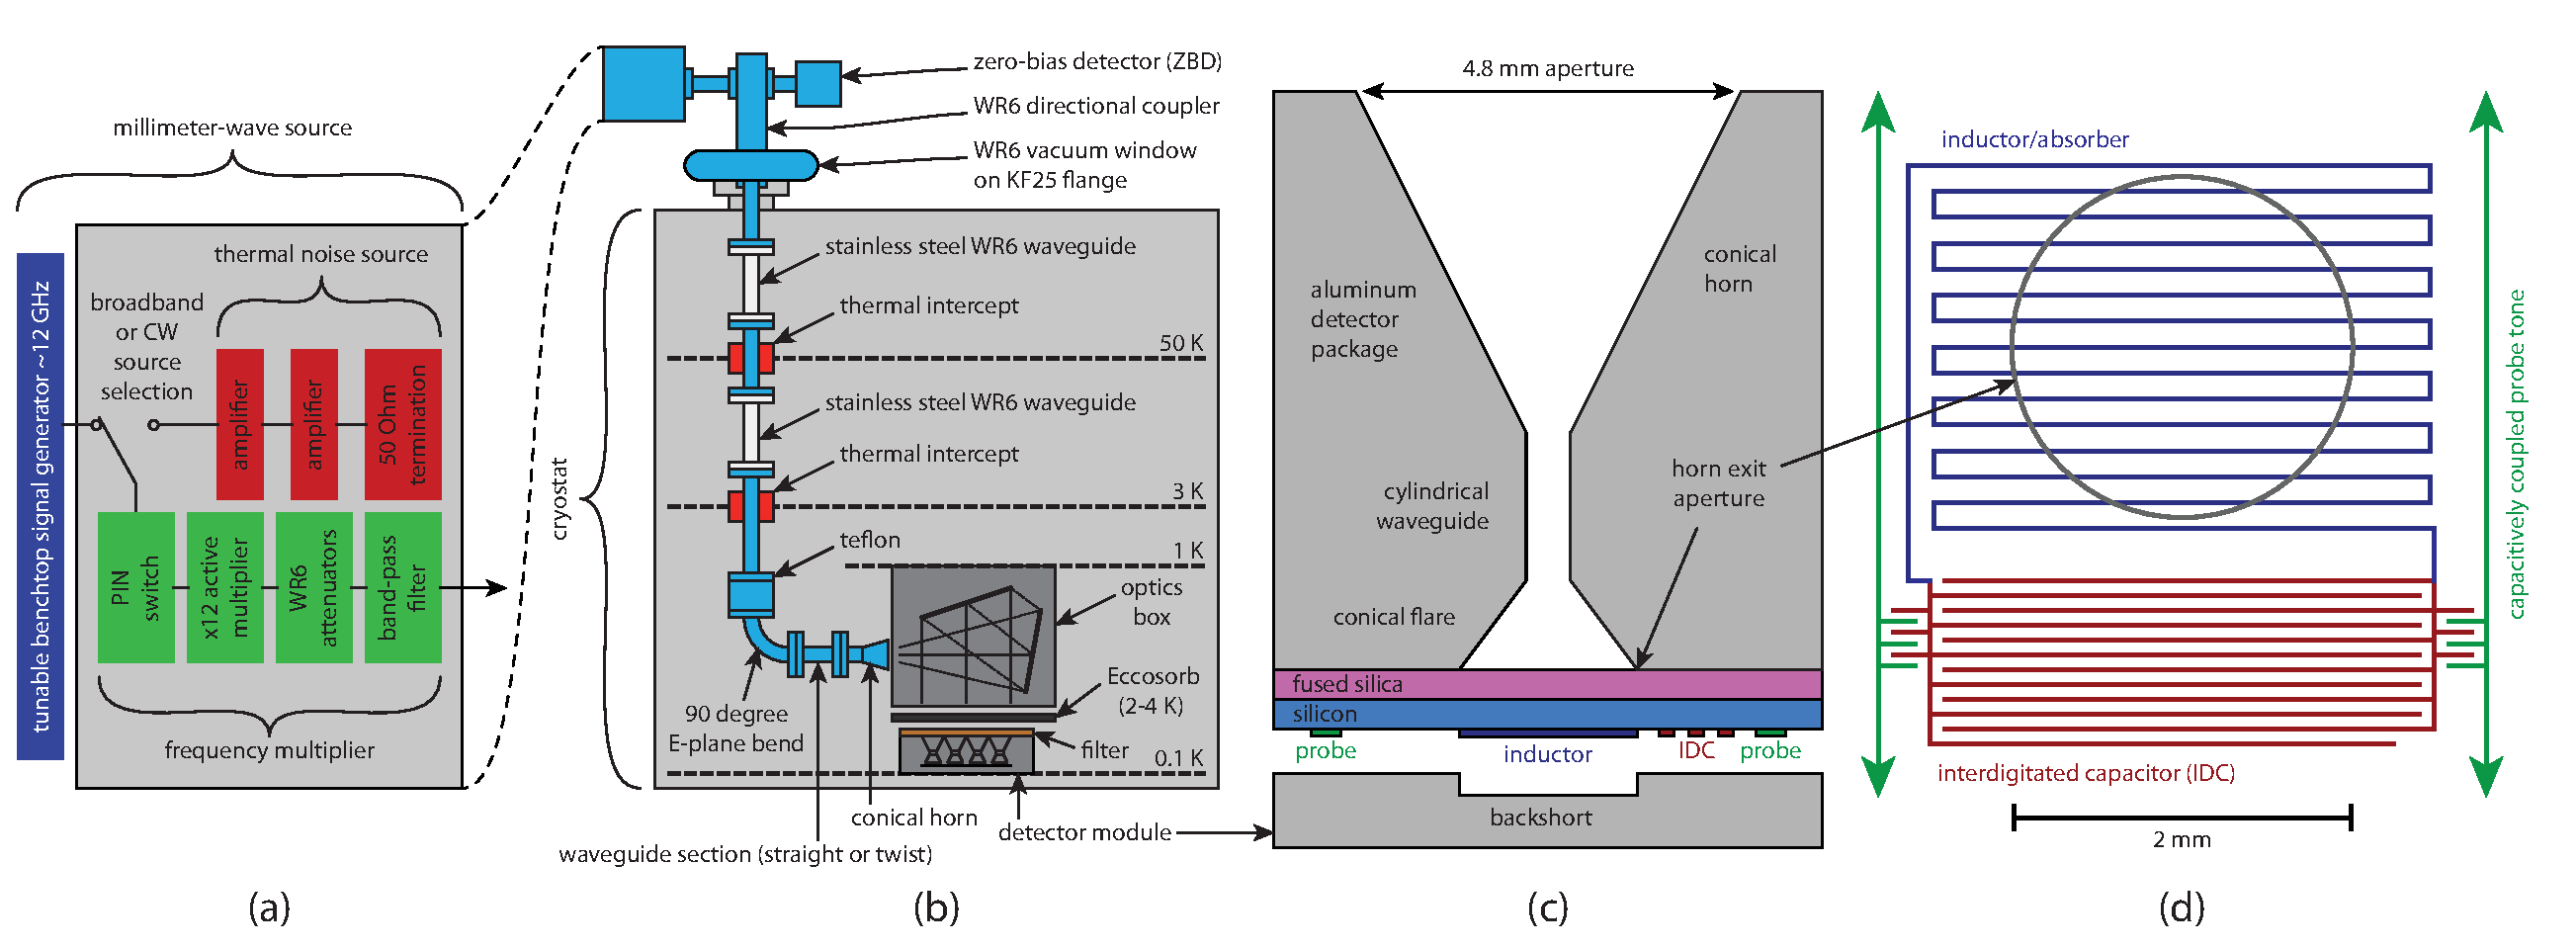
\includegraphics[width=\textwidth]{sensitivity/experiment.eps}
\caption
[Schematics of the photon noise experiment.]
{
Experiment schematics.
\textbf{(a)} The millimeter-wave source components.
\textbf{(b)} The source and cryogenic setup.
\textbf{(c)} A cross-section of an array element. The inner conical flare and fused silica layer are designed for impedance matching.
\textbf{(d)} The lumped circuit elements of one LEKID.
}
\label{fig:measuring.experiment}
\end{figure}

The array of devices used in this study was fabricated by patterning a \SI{20}{nm} aluminum film on a high-resistivity crystalline silicon substrate, with twenty detectors per array.
Each resonator comprises lithographed structures that behave electrically as lumped elements, namely an interdigitated capacitor and an inductive meander that is also the photon absorber.
Schematics of a detector and the horn coupling scheme are shown in Figure~\ref{fig:measuring.experiment}.
These devices were fabricated at STAR Cryoelectronics using the same lithographic mask used to pattern the devices described in a previous study~\autocite{McCarrick2014RSI}.
The same processing steps were used in this study except that the silicon wafer was immersed in hydrofluoric acid prior to aluminum deposition in order to clean and hydrogen-terminate the silicon surface to reduce oxide formation.
We measure a superconducting transition temperature $\tc = \SI{1.39}{K}$.
The resonance frequencies are $\SI{95}{MHz} < \freadout_\resonator < \SI{195}{MHz}$.
Under the lowest loading conditions the internal quality factors are
$\qf_\internal \approx \num{5e5} = 1 / \num{2e-6}$.
The coupling quality factors are $\qf_\coupling \approx \num{5e4} = 1 / \num{2e-5}$.
The volume of each inductive meander is \SI{1870}{\micro m^3}, assuming nominal film thickness.
The detector bath temperature is $120 \pm \SI{1}{mK}$, obtained in a cryostat using an adiabatic demagnetization refrigerator backed by a helium pulse tube cooler.
Detector readout is performed with a homodyne system using a cryogenic SiGe low-noise amplifier and open-source digital signal-processing hardware~\autocite{McCarrick2014RSI, ColumbiaCMB}.
All the data shown are from a single representative detector with $\freadout_\resonator = \SI{164}{MHz}$, and were taken at a constant readout tone power of approximately \SI{-100}{dBm} on the feedline.
The package that contains the detector chip is machined from QC-10, which is an aluminum alloy known to superconduct at the bath temperature used here.

\subsubsection{Millimeter-wave source}

Figure~\ref{fig:measuring.experiment}(a) is a schematic of the millimeter-wave source, located outside the cryostat.
Within the source, the output of a $12\times$ active multiplier chain passes through two variable waveguide attenuators that allow the output power to be controlled over a range of more than \SI{50}{dB}.
Table~\ref{tab:mmw_source} lists the primary components of the source.

The output spectrum is controlled by a band-pass filter with a sharp roll-off outside its passband of \SIrange{140}{160}{GHz}.
Within this passband, the source can produce radiation in two modes.
In \textit{broadband} mode, amplified noise is multiplied into a broadband chaotic signal.
In \textit{continuous-wave} mode, a multiplied tone from a signal generator approximates a monochromatic coherent signal.
We have measured the source output in both modes using a Fourier transform spectrometer; these measurements show that in broadband mode the power is constant within a factor of two across the output band, and in continuous-wave mode it appears monochromatic with negligible higher harmonics.

Figure~\ref{fig:measuring.experiment}(b) shows the signal path from the source through the cryostat to the detectors.
The source output is split using a waveguide directional coupler that sends 99\% of the power into a calibrated, isolator-coupled zero-bias diode power detector (ZBD), the voltage output of which is recorded using a lock-in amplifier.
The remaining 1\% of the power travels through a vacuum window and into the cryostat through WR6 waveguide.
A piece of Teflon at \SI{4}{K} inserted into the waveguide absorbs room-temperature thermal radiation.
Two mirrors transform the output of a conical horn into a collimated beam.
A \SI{6.4}{mm} thick slab of microwave absorber (Eccosorb MF-110), regulated at \SI{2}{K} during these measurements, attenuates incoming signals and provides a stable background load.
A metal-mesh filter at the detector apertures defines the upper edge of the detector band at \SI{170}{GHz}.
The lower edge of the band at \SI{130}{GHz} is defined by the cutoff frequency of a \SI{1.35}{mm} diameter circular waveguide in the detector package.
We note that the source output is within the single-mode bandwidth of both WR6 waveguide and the circular waveguide.
The radiation from the source incident on the detector horns is linearly polarized, and the electric field is aligned with the long elements of the inductive meanders in the detectors.

\begin{figure}[p]
\centering
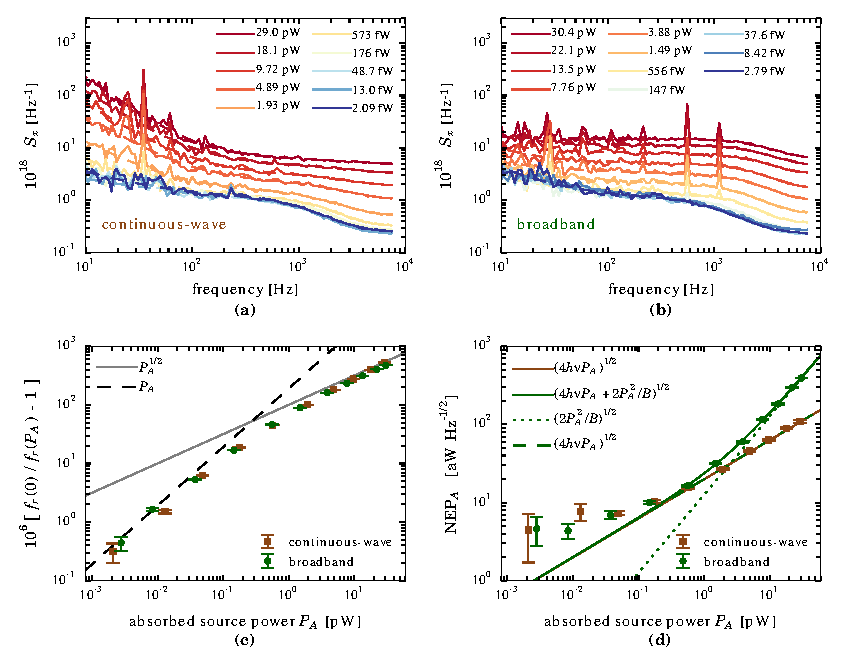
\includegraphics[width=\textwidth]{sensitivity/results.eps}
\caption
[Primary results of the photon noise experiment.]
{
Primary results of the experiment.
\textbf{(a)} Spectral density $\spectraldensity_{\detuning}$ of detector time-ordered data versus frequency under continuous-wave illumination with $\foptical = \SI{148}{GHz}$ (solid lines), and the result of fitting the data to Equation~\ref{eqn:noise_model} (dashed lines).
At high power the red noise component is dominated by fluctuations from the signal generator that feeds the multiplier; these fluctuations are correlated among detectors.
\textbf{(b)} Spectral density under broadband illumination, and fits of Equation~\ref{eqn:noise_model}.
The spikes above \SI{400}{Hz} are pickup from a fan in the source.
The red noise below \SI{100}{Hz} at low source power in both modes is produced by vibrations from the pulse tube cooler that vanish when it is turned off.
The detector white noise levels from the fits are used to calculate NEP values.
\textbf{(c)} Fractional frequency response versus absorbed power in both source modes.
The error bars are statistical errors from the resonator fits.
We use the finite-difference derivative of these response data to calculate the NEP.
The dashed black line and solid gray line are guides that show how the response scales at both low and high absorbed power.
\textbf{(d)}
Noise-equivalent power versus absorbed power in both source modes.
All data points and lines are referenced to absorbed power.
The error bars are propagated statistical errors from the finite difference derivative and the detector noise fits.
The solid green line is the sum of the quadratic and linear terms in the fit of Equation~\ref{eqn:nep} to the broadband $\nep^2$ data.
The dotted green line is the quadratic term, which is the photon wave noise contribution.
The dashed green line is the linear term, which contains equal contributions from photon shot noise and quasiparticle recombination noise.
The broadband frequency used is $\foptical = \SI{150}{GHz}$, near the band center.
The solid brown line (nearly coincident with dashed green) is the linear term in the fit of Equation~\ref{eqn:nep} to the continuous-wave $\nep^2$ data, in which the quadratic term is omitted.
}
\label{fig:measuring.results}
\end{figure}

\subsection{Results}

Figure~\ref{fig:measuring.results} shows the main results of this work.
All power values in this figure refer to the power from the source absorbed by the detector: $\power_\absorbed = \efficiency_\source \power_\source$, where $\power_\source$ is measured by the ZBD.
Before calibration, the efficiency $\efficiency_\source$ is known only approximately from measurements and simulations of the components between the source and the detector.
We accurately determine $\efficiency_\source$, and thus the absorbed source power, by measuring the relationship between emitted source power and detector noise.
This calibration relies on the assumption that all components between the source output and detector are linear: we have linearized the ZBD response at the higher power levels, all other components are passive, and we assume that filter heating is negligible.
To perform the calibration we use measurements of the noise-equivalent power (NEP), defined as the standard error of the mean in the inferred optical power at a given point in the optical system after \SI{0.5}{s} of integration~\autocite{Richards1994JAP,Zmuidzinas2003ApplOpt}.
We calculate the NEP using measurements of the detector noise and responsivity.

\subsubsection{Detector response}

At each source power level, to determine the resonance frequency and the quality factors we sweep the readout tone generator frequency $\freadout_\readout$ across a resonance and fit a resonator model to the forward scattering parameter $\forwardscattering(\freadout_\readout)$ data~\autocite{McCarrick2014RSI}.
Figure~\ref{fig:measuring.results}(c) shows the detector response to source power in both broadband and continuous-wave modes.
At low source power in both modes the fractional frequency shift
$\shift(\power_\absorbed) = \freadout_\resonator(0) / \freadout_\resonator(\power_\absorbed) - 1$ is approximately linear in power, while at high power $\shift \propto \power_\absorbed^{1/2}$.
This behavior is described by a model in which the fractional frequency shift is proportional to the number of quasiparticles:
\begin{equation}
\qpnumber
  =
  \left[ \volume (\Rate_\constant + \Rate_\source) / \qprecombinationeff \right]^{1/2},
\end{equation}
from Equation~\ref{eqn:qpnumber.response}.
Here, $\Rate_\source \propto \power_\absorbed$ is the rate of quasiparticle generation due to absorbed source photons and $\Rate_\constant$ is the constant generation rate due to other effects (such as absorption of ambient photons and thermal phonons).
We calculate the responsivity $\dv*{\detuning}{\power_\source}$ at each source power level with a finite-difference derivative that uses the fractional frequency response at adjacent power levels.


\subsubsection{Detector noise}

To measure detector noise we record time-ordered data $\forwardscattering(\freadout_\readout = \freadout_\resonator)$.
Using the resonator model from the fit to the frequency sweep we convert these data into units of detuning $\detuning$, then calculate the single-sided spectral density $\spectraldensity_{\detuning}(\faudio)$.
Figures~\ref{fig:measuring.results}(a) and \ref{fig:measuring.results}(b) show the measured noise spectra and fits to the following model:
\begin{equation}
\label{eqn:noise_model}
\spectraldensity_{\detuning}(\faudio)
  =
  \detectorwhite^2 \frac{1 + (\faudio_\knee / \faudio)^\spectralindex}{1 + (\faudio / \faudio_\cutoff)^2} + \amplifierwhite^2,
\end{equation}
where the free parameters are the detector white noise $\detectorwhite^2$, the red noise knee frequency $\faudio_\knee$, the spectral index $\spectralindex$, the cutoff frequency $\faudio_\cutoff$, and the amplifier noise $\amplifierwhite^2$.
This model treats the detector noise as the sum of a white noise process with spectral density $\detectorwhite^2$ and a red noise process with spectral density $\detectorred^2 = \detectorwhite^2 (\faudio_\knee / \faudio)^\spectralindex$, both rolled off at $\faudio_\cutoff$.

The detector bandwidth of about \SI{1}{kHz} corresponds to a limiting time constant $\tau = (2 \pi \faudio_\cutoff)^{-1}$ that is approximately equal to both the resonator ring-down time $\tau_\resonator = \qf_\resonator / \pi \freadout_\resonator$ and the expected quasiparticle relaxation time $\qprelaxationtime$ for aluminum.
Both of these time constants are expected to decrease as the absorbed optical power increases, as observed in the data.

To model the detector noise, we first consider noise sources independent of the quasiparticle system.
White noise due to the cryogenic amplifier dominates at frequencies well above the detector bandwidth, and we account for it in the model for the noise spectra.
Two-level systems (TLS) in amorphous dielectric surface layers located near the resonator produce fluctuations in the local dielectric constant and thus in $\freadout_\resonator$~\autocite{Gao2008bAPL}.
In a separate experiment, described in Section~\ref{sec:sensitivity.measuring.supplemental_material}, we determined that TLS noise is negligible at the readout power level (\SI{-100}{dBm}) used in the measurements presented here and thus do not include it in the noise model.
The chosen readout power level is high enough to suppress TLS noise but is not so high that nonlinear effects due to resonator bifurcation become significant.

The remaining noise sources involve fluctuations in the quasiparticle system: generation by optical photons, readout photons, and thermal phonons, as well as quasiparticle recombination, e.g. via phonon emission.
All of these sources are expected to produce white noise that rolls off at the frequency corresponding to the larger of $\tau_\resonator$ and $\qprelaxationtime$~\autocite{Zmuidzinas2012ARCMP}.
We expect readout generation to be negligible at high source power, and treat it as constant.
(Where present, the photon wave noise introduces correlations between photon arrival times.
This noise has a bandwidth equal to the \SI{20}{GHz} bandwidth of the absorbed broadband radiation, so it is also expected to appear white in the detector audio band~\autocite{Zmuidzinas2003ApplOpt}.)


\subsubsection{NEP model}

The NEP model includes theoretical expectations for photon noise and quasiparticle recombination noise.
We denote by $\photonoccupancy$ the mean photon occupancy of a single spatial/polarization mode of the electromagnetic field with frequency $\foptical$.
For example, for a thermal source at temperature $T$ the occupancy is
$\photonoccupancy = [\exp(\planck \foptical / \kb \temperature) - 1]^{-1}$,
where $\planck$ is Planck's constant and $\kb$ is Boltzmann's constant.
If we assume that the radiation occupies an effective optical bandwidth $\opticalbandwidth \ll \nu$ sufficiently narrow that quantities such as occupancy and absorption efficiency can be treated as constant, then the power from this mode that is absorbed by a detector with absorption efficiency $\efficiency$ is
$\power_\absorbed = \efficiency \photonoccupancy \opticalbandwidth \planck \nu$.
If the source is thermal then the contribution of photon noise to the NEP is given by~\autocite{Zmuidzinas2003ApplOpt}
\begin{equation}
\label{eqn:photon_nep}
\nep_{\absorbed, \photon}^2
  =
  2 \efficiency \photonoccupancy (1 + \efficiency \photonoccupancy) \opticalbandwidth (\planck \foptical)^2
  =
  2 \planck \foptical \power_\absorbed + 2 \power_\absorbed^2 / \opticalbandwidth,
\end{equation}
which is referenced to absorbed power.
We refer respectively to these two terms as shot noise and wave noise, following Hanbury Brown and Twiss~\autocite{HBTI1957RoyalSoc}.
If the source is monochromatic with perfect temporal coherence then only the shot noise term is present regardless of the occupancy: this behavior represents a key difference between a quantum coherent state and a quantum-statistical thermal state of the field~\autocite{Loudon2002,Glauber2006Nobel}.
For a thermal source, if $\efficiency \photonoccupancy \ll 1$ the shot noise dominates, which is typical in optical astronomy; if $\efficiency \photonoccupancy \gg 1$ the wave noise dominates, which is typical in radio astronomy.

We measure power at the output of the source and detector NEP referenced to the same point.
Referencing the photon $\nep$ to the source output gives
\begin{equation}
\label{eqn:photon_nep_source}
\nep_{\source, \photon}^2
  =
  \nep_{\absorbed, \photon}^2 / \efficiency_\source^2
  =
  2 \planck \foptical \power_\source / \efficiency_\source + 2 \power_\source^2 / \opticalbandwidth.
\end{equation}
The presence of the efficiency $\efficiency_\source$ in the linear term of this equation enables extraction of the absorbed source power.

Previous studies that calculated the absorption efficiency of a KID by measuring the scaling of photon shot noise with optical power have used superconducting films with transition temperatures similar to the film used here but larger photon energies~\autocite{Yates2011APL,Janssen2013APL,deVisser2014NatComm,Hubmayr2015APL}.
Here, the photons have energies $\planck \foptical \gtrsim 2 \gap$, where $\gap$ is the superconducting energy gap, so each photon excites only two quasiparticles close to the gap; in this limit the quasiparticle recombination noise is significant.
The recombination noise contribution to $\nep_\absorbed$ is
\begin{equation}
\label{eqn:recombination_nep}
\nep_{\absorbed, \recombination}^2
  =
  4 \gap \power_\absorbed / \pbefficiency
\end{equation}
where $\pbefficiency$ is the pair-breaking efficiency.
For photon energies $2 \gap < \planck \foptical < 4 \gap$, \textcite{deVisser2015APL} found $\pbefficiency \approx 2 \gap / \planck \foptical$, in agreement with theoretical predictions from \textcite{Guruswamy2014SUST}.
Using this value, the recombination NEP equals the shot noise term in the photon NEP.
This is expected based on the symmetry between uncorrelated pair-breaking events and uncorrelated pair-recombination events.
Finally, we introduce a small constant term $\nep_\constant$ to account for noise sources independent of source power, such as TLS noise and quasiparticle generation-recombination noise from thermal phonons, readout photons, and ambient photons.

To calculate the detector $\nep_\absorbed$, which is shown in Figure~\ref{fig:measuring.results}(d), we use the measured fractional frequency shift $\detuning$ (unitless), the measured fractional frequency noise power $\spectraldensity_{\detuning}$ (1 / Hz), and the source power $\power_\source$ (watts) as measured with a calibrated zero-bias diode (ZBD) mounted on the directional coupler outside the cryostat (see Figure 1).
The source power absorbed by the detector is related to $\power_\source$ by $\power_\absorbed = \efficiency_\source \power_\source$ where $\efficiency_\source$ is an overall system efficiency from the source output to the detector that includes the transmission through the directional coupler, the attenuation of the stainless steel waveguide, the geometrical dilution due to the internal optics, the loss in the Eccosorb, and the detector absorption efficiency.
To compute the responsivity to changes in the source power, we plot $\detuning$ versus $\power_\source$ and calculate the slope of this curve $\dv*{\detuning}{\power_\source}$ at each $\power_\source$ using a finite difference algorithm.
We use this responsivity to convert the fractional frequency noise measurements ($\spectraldensity_{\detuning}$) to $\nep_\source$.
Note that for $\nep_\source$ we use only the white noise component, $\detectorwhite$, obtained by fitting Equation~\ref{eqn:noise_model} to each $\spectraldensity_{\detuning}$ measurement.
Thus, $\nep_\source = \detectorwhite / (\dv*{\detuning}{\power_\source})$.
To convert $\power_\source$ to $\power_\absorbed$ we need to determine $\efficiency_\source$.
The complete theoretical model for $\nep_\source$ is
\begin{align}
\begin{split}
\label{eqn:nep}
\nep_\source^2
  &=
  (\nep_{\absorbed, \constant}^2
   + \nep_{\absorbed, \recombination}^2
   + \nep_{\absorbed, \photon}^2) / \efficiency_\source^2 \\
  &=
  \nep_{\absorbed, \constant}^2 / \efficiency_\source^2
  + [2 (2 \planck \foptical \power_\absorbed) + 2 \power_\absorbed^2 / \opticalbandwidth] / \efficiency_\source^2 \\
  &=
  \nep_{\source, \constant}^2
  + 4 \planck \foptical \power_\source / \efficiency_\source
  + 2 \power_\source^2 / \opticalbandwidth,
\end{split}
\end{align}
which is the sum of the aforementioned noise contributions.
The right-hand side of this equation is quadratic in $P_\source$ with unknown quantities $\nep_{\source, \constant}$, $\efficiency_\source$, and effective optical bandwidth $\opticalbandwidth$.
The limiting $\nep_{\source, \constant}$ is discussed below.
We fit Equation~\ref{eqn:nep} to the broadband data using center frequency $\foptical = \SI{150}{GHz}$ and obtain $\efficiency_\source = \num{8.50e-7} (1 \pm 0.09)$ and $\opticalbandwidth = \SI{13}{GHz}$.
The quadratic term is not expected to be present for coherent illumination because the source should produce only shot noise, so we fit Equation~\ref{eqn:nep} to the continuous-wave data omitting the third term.
Here, $\foptical = \SI{148}{GHz}$ and we obtain $\efficiency_\source = \num{1.12e-6} (1 \pm
0.04)$.
As a final step, we convert $\power_\source$ to $\power_\absorbed$ using the $\efficiency_\source$ values from the model fitting and produce Figures~\ref{fig:measuring.results}(c) and \ref{fig:measuring.results}(d).
Note that because the broadband source involves contributions from the full source output bandwidth, it is not surprising that the measured $\efficiency_\source$ values differ between the continuous-wave and broadband modes by more than the statistical error bars.

\subsection{Discussion}

Figure~\ref{fig:measuring.results}(d) shows that photon noise dominates under broadband illumination when
$\power_\absorbed \gtrsim \SI{1}{pW}$,
which corresponds to 
$\nep_\absorbed \approx \SI{2e-17}{W.Hz^{-1/2}}$.
At high power in each source mode we observe the expected relationship between noise and power: in broadband mode $\nep \propto \power$ because the quadratic wave noise term dominates, while in continuous-wave mode $\nep \propto \power^{1/2}$ because the quadratic term is not present.
This behavior is a clear signature of photon noise.

Note that the the $\nep_\absorbed$ values reported have the amplifier noise contribution subtracted because the white noise parameter $W^2$ in Equation~\ref{eqn:noise_model} describes the noise power above the amplifier noise $\amplifierwhite^2$.
Here, subtracting the amplifier noise yields an accurate estimate of the detector performance because, alternatively, the amplifier noise can be suppressed to a negligible level by increasing the readout power.
We verified both approaches yield the same $\nep_\absorbed$ versus $\power_\absorbed$ result but chose to report the amplifier-noise-subtracted results.

At low absorbed source power levels in both modes, where $\power_\absorbed < \SI{0.1}{pW}$, $\nep_\absorbed$ levels off to $\nep_\constant$.
The values of $\nep_\constant$ extracted from both of the aforementioned fits are approximately 5 to \SI{6e-18}{W.Hz^{-1/2}}.
To explain this leveling-off effect, we model the background loading as emission from a black body at \SI{2}{K}, which is the temperature of the Eccosorb in front of the feed horn apertures.
Assuming center frequency $\foptical = \SI{150}{GHz}$, measured filter transmission $\efficiency_\mathrm{F}(\nu) = 0.94$, optical efficiency $\efficiency_\incident = 0.7$ (obtained from electromagnetic simulations), and detector bandwidth $\opticalbandwidth_\mathrm{full} = \SI{40}{GHz}$, then the radiative loading from the Eccosorb is 
\begin{equation*}
\power_\absorbed
  =
  \efficiency_\incident \photonoccupancy(\foptical, \SI{2}{K}) \planck \foptical \opticalbandwidth_\mathrm{full} = \SI{0.08}{pW}.
\end{equation*}
This loading level is close to the observed knee in the curves in Figure~\ref{fig:measuring.results}(d).
Adding an equal recombination noise contribution to the corresponding photon NEP results in
\begin{equation}
\nep_\absorbed = (2 \cdot 2 \planck \foptical \power_\absorbed)^{1/2} = \SI{5.6e-18}{W.Hz^{-1/2}},
\end{equation}
which is close to the observed $\nep_\constant$ value.
Therefore, the observed limiting $\nep_\absorbed$ is consistent with this model of the expected background loading.

Analysis of data from twelve detectors yielded similar results to those shown in Figure~\ref{fig:measuring.results}(d), with the photon noise starting to dominate between 0.5 and \SI{1}{pW}.
We conclude that these detectors become limited by photon noise at absorbed power levels lower than the background power levels already measured by ground-based CMB polarimeters~\autocite{BICEP2II2014ApJ}.


\subsection{Supplemental material}
\label{sec:sensitivity.measuring.supplemental_material}

The contents of this section were presented as supplemental material for the published paper.
The content that is specific to the paper is retained here, while the more general content has been moved earlier in this chapter.

\subsubsection{Two-level system noise}

At low temperatures we see evidence for TLS effects in measurements of resonance frequency versus bath temperature, which depart from the Mattis-Bardeen prediction, and in the fact that the internal quality factors increase with increasing readout power.
The connection between these steady-state TLS effects and TLS noise is not fully understood.
The method we used to estimate the TLS noise contribution is described in this section.
We conclude that TLS noise is negligible and thus do not include it explicitly in the analysis of the NEP.

The importance of modeling TLS noise to avoid a systematic error in this measurement is explained in Section~\ref{sec:sensitivity.tls}.
The TLS contribution to the spectral density is given by 
Equation~\ref{eqn:spectraldensity_tls}.
The experiment described in the main text is performed with constant readout power $\power_\readout$ on the feedline, and we expect the TLS noise level to vary as $\power_\internal^{-1/2} = (\chi_a \power_\readout)^{-1/2}$, where $\chi_a \le 1/2$, which can be calculated from the resonator parameters, is the fraction of readout power that flows into the resonator~\autocite{Zmuidzinas2012ARCMP}.

\begin{figure}[htb]
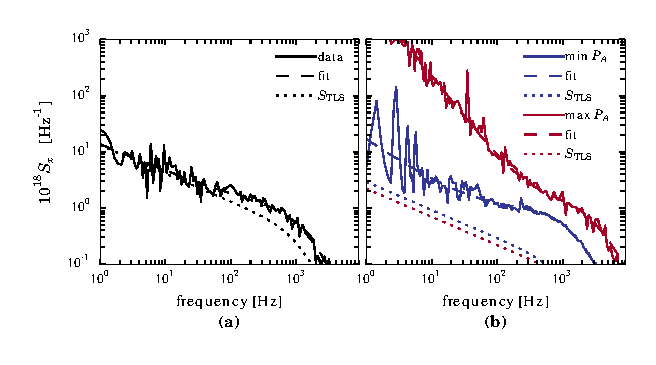
\includegraphics[width=\columnwidth]{sensitivity/dark_and_light_noise_minus_amp_two_panel.eps}
\caption
[Dark noise data and fits.]
{
\textbf{(a)}
Amplifier-subtracted dark noise data for the same detector characterized in the main text.
The dashed line shows a fit to the same model used in the main text, except that here the spectral index is fixed to $\spectralindex = 0.5$ to match a possible TLS contribution.
To show the detector noise more clearly, the amplifier noise value obtained from the fit has been subtracted from the data and fit curves.
The dotted line shows the possible TLS contribution, assumed to roll off with the same time constant obtained from the fit.
\textbf{(b)}
Amplifier-subtracted illuminated continuous-wave noise data.
The solid lines shown here are the lowest and highest power curves from Figure~\ref{fig:measuring.results}(a), and the dashed lines are the same fits shown in the main text, except that the amplifier noise values obtained from the fits have been subtracted from the data and fit curves.
The dotted lines are the inferred TLS contribution to the illuminated spectra, scaled from the fit value in panel (a) by a factor $(\power_{\internal, \dark} / \power_\internal)^{1/2}$.
The TLS contribution in this case decreases as source power increases.}
\label{fig:measuring.dark_noise}
\end{figure}

In order to estimate the TLS contribution to the NEP, we performed a separate experiment in which we attempted to make the TLS noise as prominent as possible.
Three key aspects differ from the experiment described in the main text: the horn apertures were covered with aluminum tape to minimize optical loading; the readout power was approximately \SI{-112}{dBm}, \SI{12}{dB} lower than in the primary experiment; in order to remove noise due to vibrations caused by the pulse tube cooler, we turned it off to record time-ordered data while the adiabatic demagnetization refrigerator continued to regulate the bath temperature at \SI{120}{mK}.

Figure~\ref{fig:measuring.dark_noise}(a) shows the detuning spectral density taken under these dark conditions and a fit used to extract a possible TLS noise contribution.
Figure~\ref{fig:measuring.dark_noise}(b) shows that this TLS contribution is negligible when adjusted for the increased readout power used in the primary experiment.


\subsubsection{Spectral density fitting}

\begin{table}[htb]
\centering
\caption
[Best-fit parameters from the spectral density fits of the broadband data.]
{Broadband best-fit parameters with uncertainties.
At high power, because the noise is very close to white, the red noise contribution is negligible and the parameters ($\faudio_\knee$ and $\spectralindex$) that describe the red noise are poorly constrained; the white noise $\detectorwhite^2$ is still well constrained.}
\renewcommand{\arraystretch}{1.2}
\begin{tabular}{cccccc}
\toprule
$\power_\absorbed$ & $\amplifierwhite^2 / \SI{e-18}{Hz^{-1}}$ & $\detectorwhite^2 / \SI{e-18}{Hz^{-1}}$ & $\faudio_\knee / \si{Hz}$ & $\spectralindex$ & $\faudio_\cutoff / \si{kHz}$ \\
\midrule
\SI{30.4}{pW} & 5.2 $\pm$ 0.1 & 10.0 $\pm$ 0.2 & 0 $\pm$ 20 & 1 $\pm$ 6 & 3.0 $\pm$ 0.1 \\
\SI{22.1}{pW} & 3.9 $\pm$ 0.1 & 7.7 $\pm$ 0.1 & 11 $\pm$ 3 & 1.9 $\pm$ 0.9 & 2.9 $\pm$ 0.1 \\
\SI{13.5}{pW} & 2.67 $\pm$ 0.06 & 5.3 $\pm$ 0.1 & 7 $\pm$ 4 & 1.0 $\pm$ 0.5 & 2.7 $\pm$ 0.1 \\
\SI{7.76}{pW} & 1.38 $\pm$ 0.03 & 3.81 $\pm$ 0.08 & 12 $\pm$ 3 & 1.2 $\pm$ 0.4 & 2.48 $\pm$ 0.08 \\
\SI{3.88}{pW} & 0.82 $\pm$ 0.02 & 2.4 $\pm$ 0.1 & 9 $\pm$ 4 & 0.8 $\pm$ 0.3 & 2.34 $\pm$ 0.10 \\
\SI{1.49}{pW} & 0.481 $\pm$ 0.007 & 1.73 $\pm$ 0.05 & 14 $\pm$ 3 & 1.2 $\pm$ 0.3 & 1.80 $\pm$ 0.05 \\
\SI{556}{fW} & 0.309 $\pm$ 0.005 & 1.11 $\pm$ 0.04 & 13 $\pm$ 3 & 1.0 $\pm$ 0.3 & 1.70 $\pm$ 0.06 \\
\SI{147}{fW} & 0.229 $\pm$ 0.002 & 0.98 $\pm$ 0.03 & 21 $\pm$ 2 & 1.2 $\pm$ 0.2 & 1.29 $\pm$ 0.03 \\
\SI{37.6}{fW} & 0.201 $\pm$ 0.002 & 0.69 $\pm$ 0.09 & 60 $\pm$ 20 & 0.7 $\pm$ 0.1 & 1.24 $\pm$ 0.07 \\
\SI{8.42}{fW} & 0.247 $\pm$ 0.002 & 0.77 $\pm$ 0.08 & 60 $\pm$ 20 & 0.7 $\pm$ 0.1 & 1.14 $\pm$ 0.05 \\
\SI{2.79}{fW} & 0.213 $\pm$ 0.002 & 0.89 $\pm$ 0.05 & 34 $\pm$ 5 & 1.0 $\pm$ 0.2 & 1.06 $\pm$ 0.04 \\
\bottomrule
\end{tabular}
\label{tab:bbfitparams}
\end{table}

\begin{table}[t]
\centering
\caption
[Best-fit parameters from the spectral density fits of the continuous-wave data.]
{Continuous-wave best-fit parameters with uncertainties.}
\renewcommand{\arraystretch}{1.2}
\begin{tabular}{cccccc}
\toprule
$\power_\absorbed$ & $\amplifierwhite^2 / \SI{e-18}{Hz^{-1}}$ & $\detectorwhite^2 / \SI{e-18}{Hz^{-1}}$ & $\faudio_\knee / \si{Hz}$ & $\spectralindex$ & $\faudio_\cutoff / \si{kHz}$ \\
\midrule
\SI{29.0}{pW} & 4.89 $\pm$ 0.06 & 1.3 $\pm$ 0.1 & 330 $\pm$ 40 & 1.46 $\pm$ 0.05 & 2.5 $\pm$ 0.4 \\
\SI{18.1}{pW} & 3.20 $\pm$ 0.04 & 1.46 $\pm$ 0.09 & 270 $\pm$ 30 & 1.33 $\pm$ 0.05 & 2.6 $\pm$ 0.3 \\
\SI{9.72}{pW} & 1.82 $\pm$ 0.03 & 1.27 $\pm$ 0.07 & 220 $\pm$ 30 & 1.28 $\pm$ 0.06 & 2.4 $\pm$ 0.2 \\
\SI{4.89}{pW} & 0.98 $\pm$ 0.01 & 1.22 $\pm$ 0.05 & 160 $\pm$ 20 & 1.25 $\pm$ 0.06 & 2.2 $\pm$ 0.1 \\
\SI{1.93}{pW} & 0.462 $\pm$ 0.006 & 0.97 $\pm$ 0.04 & 100 $\pm$ 10 & 1.09 $\pm$ 0.07 & 1.83 $\pm$ 0.07 \\
\SI{573}{fW} & 0.288 $\pm$ 0.003 & 0.87 $\pm$ 0.04 & 52 $\pm$ 7 & 1.1 $\pm$ 0.1 & 1.56 $\pm$ 0.05 \\
\SI{176}{fW} & 0.244 $\pm$ 0.003 & 0.88 $\pm$ 0.06 & 37 $\pm$ 8 & 0.9 $\pm$ 0.2 & 1.29 $\pm$ 0.05 \\
\SI{48.7}{fW} & 0.219 $\pm$ 0.002 & 0.82 $\pm$ 0.05 & 39 $\pm$ 7 & 1.0 $\pm$ 0.1 & 1.21 $\pm$ 0.05 \\
\SI{13.0}{fW} & 0.210 $\pm$ 0.002 & 0.7 $\pm$ 0.2 & 40 $\pm$ 40 & 0.6 $\pm$ 0.2 & 1.17 $\pm$ 0.08 \\
\SI{2.09}{fW} & 0.235 $\pm$ 0.002 & 0.85 $\pm$ 0.08 & 40 $\pm$ 10 & 0.8 $\pm$ 0.2 & 1.13 $\pm$ 0.05 \\
\bottomrule
\end{tabular}
\label{tab:cwfitparams}
\end{table}

In this section we provide details of the procedure used to fit the spectral density to Equation~\ref{eqn:noise_model}.
To estimate the spectral density of the time-ordered fractional frequency shift data we first use Welch's average periodogram method with the data split into 16 equal non-overlapping chunks.
This produces a single-sided spectral density that is the average of 16 spectra.
We estimate the variance of point $j$ with value $\spectraldensity_j$ by $\sigma_j^2 = \spectraldensity_j^2 / 16$.
We then bin this spectrum using bin widths that increase with frequency, and propagate the errors by adding the variances in quadrature.
These binned spectra are plotted in Figures~\ref{fig:measuring.results}(a) and \ref{fig:measuring.results}(b).

This binning and averaging procedure produces $\chi^2$ distributed data with $2 \times 16 \times n_k$ degrees of freedom, where $n_k$ is the number of points that are averaged in bin $k$.
The resulting distribution closely approximates a Gaussian distribution~\autocite{Norrelykke2010RSI}, even for $n_k = 1$.
To fit the model to the data we use a least-squares fitting routine with the squared residual at each frequency point weighted by the inverse of the variance in that bin.
Only data at frequencies above \SI{10}{Hz} is used in the fits.
This model will over-describe the data if the spectrum has no red noise or no white noise component, in which case the uncertainties on the remaining parameters would be underestimated.
The resulting best-fit parameters are listed in Tables~\ref{tab:bbfitparams}~and~\ref{tab:cwfitparams}.
